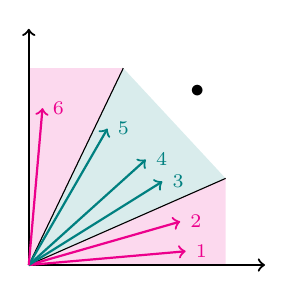
\begin{tikzpicture}
    \coordinate (A) at (0,0);
    \coordinate (B) at (0,3);
    \coordinate (C) at (3,3);
    \coordinate (D) at (3,0);
    \coordinate (E) at (2.5,1.1);
    \coordinate (F) at (1.2,2.5);

    \path[fill=magenta!15] (A) to (E) -- (2.5,0) to (A);
    \path[fill=magenta!15] (A) to (F) -- (0,2.5) to (A);
    \path[fill=teal!15] (A) to (F) -- (E) to (A);

    \draw (A) -- (E);
    \draw (A) -- (F);
    \draw[thick,->] (A) -- (B);
    \draw[thick,->] (A) -- (D);

    \draw[thick, magenta, ->] (A) -- (5:2) node[right] {$\atom_1$};
    \draw[thick, magenta, ->] (A) -- (16:2) node[right] {$\atom_2$};
    \draw[thick, teal, ->] (A) -- (32:2) node[right] {$\atom_3$};
    \draw[thick, teal, ->] (A) -- (42:2) node[right] {$\atom_4$};
    \draw[thick, teal, ->] (A) -- (60:2) node[right] {$\atom_5$};
    \draw[thick, magenta, ->] (A) -- (85:2) node[right] {$\atom_6$};
    \draw[circle] (2.2, 2.2) node {$\bullet \ \opt{\dv}$};

\end{tikzpicture}